\documentclass[crop, tikz]{standalone}
\usepackage{tikz}
\usepackage{tkz-graph}

\begin{document}
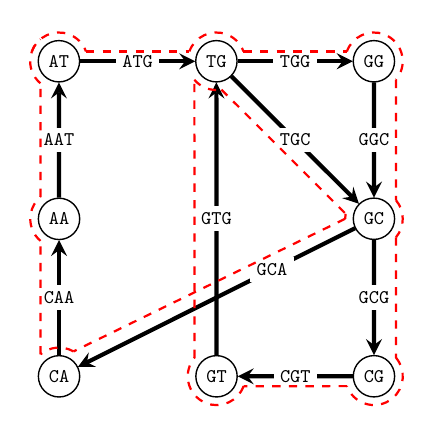
\begin{tikzpicture}[scale=0.8,every node/.style={scale=0.7},font=\tt]
	\SetUpEdge[lw         = 1.5pt,
				color      = black,
				labelcolor = white]
	\GraphInit[vstyle=Normal] 
	\SetGraphUnit{2.5}
	\tikzset{VertexStyle/.append  style={fill}}
	\Vertex{AT}
	\EA(AT){TG}
	\EA(TG){GG}
	\SO(GG){GC}
	\SO(GC){CG}
	\WE(CG){GT}
	\WE(GT){CA}
	\NO(CA){AA}
	\tikzset{EdgeStyle/.style={-stealth}}
	\Edge[label=ATG](AT)(TG)
	\Edge[label=TGG](TG)(GG)
	\Edge[label=GGC](GG)(GC)
	\Edge[label=GCG](GC)(CG)
	\Edge[label=CGT](CG)(GT)
	\Edge[label=GTG](GT)(TG)
	\Edge[label=TGC](TG)(GC)
	\Edge[label=GCA, style={pos=.3}](GC)(CA)
	\Edge[label=CAA](CA)(AA)
	\Edge[label=AAT](AA)(AT)
  
	\draw[thick, red, dashed] (AT) ++(160:13pt)coordinate(AT1)  arc (-200:-340:13pt)   coordinate(AT2);
	\draw[thick, red, dashed] (TG) ++(160:13pt)coordinate(TG1)  arc (-200:-340:13pt)   coordinate(TG2);
	\draw[thick, red, dashed] (GG) ++(160:13pt)coordinate(GG1)  arc (-200:-400:13pt)   coordinate(GG2);
	\draw[thick, red, dashed] (GC) ++(40:13pt)coordinate(GC1)  arc (-320:-400:13pt)   coordinate(GC2);
	\draw[thick, red, dashed] (CG) ++(40:13pt)coordinate(CG1)  arc (-320:-520:13pt)   coordinate(CG2);
	\draw[thick, red, dashed] (GT) ++(-20:13pt)coordinate(GT1)  arc (-380:-580:13pt)   coordinate(GT2);
	\draw[thick, red, dashed] (TG) ++(-140:13pt)coordinate(TG11)  arc (-500:-440:13pt)   coordinate(TG12);
	\draw[thick, red, dashed] (GC) ++(-550:13pt)coordinate(GC11)  arc (-550:-540:13pt)   coordinate(GC12);
	\draw[thick, red, dashed] (CA) ++(-660:13pt)coordinate(CA1)  arc (-660:-590:13pt)   coordinate(CA2);
	\draw[thick, red, dashed] (AA) ++(-490:13pt)coordinate(AA1)  arc (-490:-590:13pt)   coordinate(AA2);
	\draw[thick, red, dashed] (AT) ++(-490:13pt)coordinate(AT11)  arc (-490:-590:13pt)   coordinate(AT12);
  
	\draw[thick, red, dashed, rounded corners=3mm] (AT2) --(TG1);
	\draw[thick, red, dashed, rounded corners=3mm] (TG2) --(GG1);
	\draw[thick, red, dashed, rounded corners=3mm] (GG2) --(GC1);
	\draw[thick, red, dashed, rounded corners=3mm] (GC2) --(CG1);
	\draw[thick, red, dashed, rounded corners=3mm] (CG2) --(GT1);
	\draw[thick, red, dashed, rounded corners=3mm] (GT2) --(TG11);
	\draw[thick, red, dashed, rounded corners=3mm] (TG12) --(GC11);
	\draw[thick, red, dashed, rounded corners=3mm] (GC12) --(CA1);
	\draw[thick, red, dashed, rounded corners=3mm] (CA2) --(AA1);
	\draw[thick, red, dashed, rounded corners=3mm] (AA2) --(AT11);
\end{tikzpicture}
\end{document}
